\documentclass{article}
\usepackage{amsmath}
\usepackage{graphicx}
\usepackage{geometry}[margin=2cm]
\usepackage{example}
\usepackage{titlesec}

\title{PHY224 Curve Fit Lab 1}
\author{Hachem Fattouh}
\date{\today}

\titleformat{\title}
  {\normalfont\LARGE\bfseries} % Change \LARGE to the desired size, e.g., \large, \Large, \small, etc.
  {}
  {0pt}
  {}

\title{PHY224 Curve Fit Lab 1}
\author{Hachem Fattouh}
\date{\today}

\begin{document}

\maketitle

in exercise 1, we are given climate data containing the mean atmospheric CO2 content over the last half-century. using this data in a CSV file I plotted the data
for the last 20 years, along with a line of best fit using the linear regression line \(f(x) = ax + b\).

\begin{figure}[h]
    \centering
    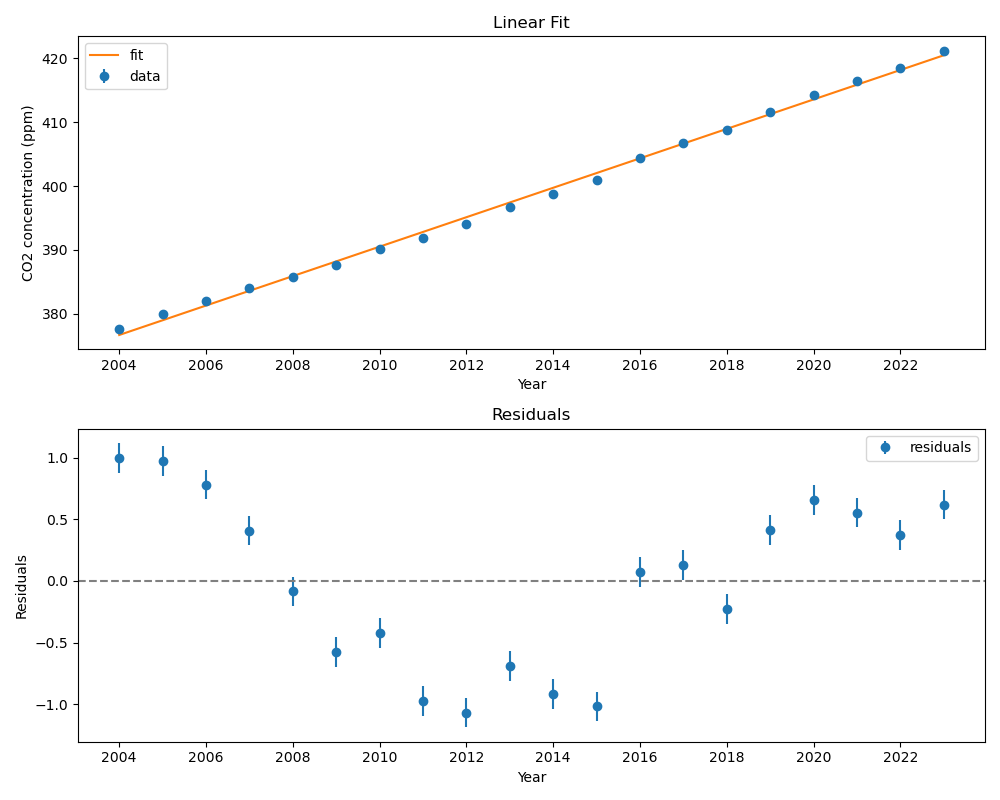
\includegraphics[width=\textwidth]{Exercise 1.png} 
    \caption{the 2 figures above are the data with its line of best fit,
    and the corresponding residuals for each dataset.}
    \label{fig:fit_and_residuals}
\end{figure}


from the data, the coefficients calculated were:
\[a = 2.303\]
\[b = -4239\]
\[r^2 = 0.997\]
\end{document}
